 \documentclass{article} %A4
\usepackage[a4paper,left=1.9cm, right=2.1cm,top = 1.2cm,bottom=2.3cm]{geometry}
\usepackage[utf8]{inputenc}%Umlaute
\usepackage[ngerman]{babel} %Texttrennung
\usepackage{graphicx}	%Grafiken
\usepackage{amssymb}
\usepackage{amsmath}
\usepackage{url}
\usepackage{listings}
 \usepackage{color}
\usepackage{hyperref}
\usepackage{framed}
\usepackage{algpseudocode}
\usepackage{tikz}

\usepackage[labelformat=empty]{caption}
\title{Zusammenfassung - NASS}
\author{
	SK
}

\begin{document}
\maketitle
\begin{framed}
	Korrektheit und Vollständigkeit der Informationen wird nicht gewährleistet.
\end{framed}
\setcounter{tocdepth}{1}
\tableofcontents

\section{Introduction}
\subsection{Taxonomie der Angreifer}
\begin{itemize}
	\item einzelner Angreifer
    
    \begin{itemize}
        \item sozialer Hintergrund
        \item öffentliche Aufmerksamkeit als Antrieb
        \item evtl pol. Statements
        \item geht gewöhnlich niedrige Risiken ein
    \end{itemize}
    \item organisierte Kriminalität
    
    \begin{itemize}
        \item Geld als Antrieb
        \item mittlere Risiken
    \end{itemize}
    \item Terroristen
    
    \begin{itemize}
        \item politische oder gesellschaftliche Motivation
        \item hohe Risiken
        \item Zerstörung/Verwirrung als Ziel
    \end{itemize}
    
    \item Konkurrenten
    
    
    \begin{itemize}
        \item möglichst niedriges Risiko der Aufdeckung(abhängig vom wert der Information)
        \item Informationsdiebstahl oder Zerstörung als Ziel
    \end{itemize}
    
    \item Regierungsorganisationen
    
    
    \begin{itemize}
        \item Industriespionage zum Wohl einheimischer Firmen
        \item Militärspionage udn hybride Kriegsführung
    \end{itemize}
\end{itemize}

\subsection{Angriffe gegen einen Computer}
Informationsdiebstahl führt zu:
\begin{itemize}
	\item Wettbewerbsvorteilen
    \item Verwirrung
    \item Erpressung
    
\end{itemize}
Zerstörung führt zu:
\begin{itemize}
	\item Spaß und Selbstverherrlichung
    \item Politischen Stellungnahmen
\end{itemize}
Sammlung von Informationen
\begin{itemize}
	\item Infos werden zu Angreifer gesendet
    \item an Netzwerk angeschlossene Rechner mit höherem Risiko
    \item Zugriff für Angreifer durch:
    
    \begin{itemize}
        \item Social engineering
        \item Viren/Trojaner/Würmer
        \item Physischer Diebstahl von Datenträgern
        \item Sniffing
    \end{itemize}
    
\end{itemize}
Zerstörung von Infos
\begin{itemize}
	\item Infos gehen verloren
    \item physische Angriffe/Feuer/Naturkatastrophen
    \item Beabsichtigte Löschungen durch 
    
    \begin{itemize}
        \item Social Engineering
        \item Viren/Trojaner/Würmer
    \end{itemize}
\end{itemize}
Viren
\begin{itemize}
	\item Infektion von Dateien 
    \item Infektion von System und Boot record
    \item Zerstörung, Verwirrung und öffentliche Aufmerksamkeit als Ziel
\end{itemize}
Würmer
\begin{itemize}
	\item Mailing Worms - Verbreitung durch E-Mails
    \item Viren/Trojaner evtl als "`Nutzlast"'
    \item Network worms - Verbreitung durch Ausnutzung von Softwaremängeln(bspw Bufferoverflows)
    \item Ablauf:
    
    \begin{itemize}
        \item Zielauswahl
        \item ausnutzen(exploit)
        \item Infektion
        \item Verbreitung
    \end{itemize}
\end{itemize}
Backdoors und Trojaner
\begin{itemize}
	\item Schadsoftware wird in nützlicher Software versteckt
    \item mögliche Funktionen:
    
    \begin{itemize}
        \item mitschneiden von Daten(logging)
        \item Zerstörung
        \item Installation weiterer Software(DoS Clients, root kits etc)
        \item bedingter Start von Prozessen (time bombs)
    \end{itemize}
\end{itemize}
Identitäts Spoofing
\begin{itemize}
	\item Angreifer übernimmt die Identität von jemand anderem 
    \item Angreifer und Ziel müssne normalerweise ein Netzsegment teilen
    \item Angreifer liefert evtl falsche Infos über Routen oder Namen
    \item Grundsätzlich sind alle Antworten eines Protokolls potentielle Spoofingsubjekte(subject of spoofing?)
\end{itemize}
DoS
\begin{itemize}
	\item Angreifer möchte einen Dienst der von einem Rechner oder Gerät angeboten wird überladen
    \item Angriffe gegen Konkurrenten, als pol/gesellschaftliche Aussage oder um andere Aktivitäten zu verbergen
    \item bösartige Anfragen sind nicht von normalen Anfragen zu unterscheiden
    \item BSP: HTTP, DNS DoS, SYN Flooding
\end{itemize}
Bot Network
\begin{itemize}
	\item Fernsteuerung mehrerer Rechner um bösartige Aktionen auszuführen
    \item bsp: DDoS, aufwändige Entschlüsselungen berechnen
\end{itemize}
Password/Schlüssel Attacken
\begin{itemize}
	\item Brute Force
    \item Raten/ Wörterbuchangriffe
    \item Mängel in der Implementation(z.B. Password als Klartext gespeichert)
\end{itemize}
Port/Network Scanning

\begin{itemize}
	\item während der Aufklärungsphase um Sicherheitslücken und geeignete Ziele zu finden
    \item Angreifer möchte Informationen über das System erlangen
    \item Sniffing/Mapping/Port Scans
\end{itemize}
Session Highjacking
\begin{itemize}
	\item Angreifer bricht in einen bestehender Session ein ohne sich einloggen zu müssen.
\end{itemize}

ZSF: viele unterschiedliche Angriffsmöglichkeiten \Rightarrow unüberschaubare Anzahl an verschiedenen Attacken
Angreifer unterscheiden sich in Motivation und Möglichkeiten.
\section{Einführung und Rekapitulation}
\subsection{Sicherheitskomponenten}
\begin{itemize}
	\item Firewalls
    \item Intrusion Detection/Prevention Systems
    \item Proxies
    \item interne oder private Netzwerke / Netzwerkzonen / Entmilitarisierte Zonen
    \item VPNs
\end{itemize}
\subsection{Firewalls}
entscheidet ob Verkehr ins Netzwerk gelangen darf oder nicht
Typen: 
\begin{itemize}
	\item Paketfilter
    \item Zustandsbehaftete Firewall
    \item Proxyfirewall
\end{itemize}
\subsection{Intrusion Detection Systems}
Identifizierung von Attacken / verdächtigem Verkehr \\
Hilfe beim Einrichten/ konfigurieren von Firewalls \\
Normalerweise transparent für Nutzer und Angreifer.\\
hauptsächlich 2 Arten:
\begin{itemize}
	\item Mustererkennung
    \item Anomalieerkennung
\end{itemize}
\subsection{Proxies}
strickte Trennung von internen und externen Netz\\
Üblicherweise auf Application Layer. Verhindert dass bestimmte Informationen(Viren, Pornos, illegale Infos) in das interne Netz gesandt werden.\\
Verhindert, dass bestimmte Informationen nach außen gesendet werden.\\
Kombinationen mit anderen Systemen(Virenfilter/ Spamfilter / IDS...)\\
\subsection{VPN}
VPNs erschaffen einen gemeinsamen Addressraum.\\
VPNs schützen die Kommunikation über ungesicherte Netzwerke als würde sie in einem Netzwerk stattfinden.\\
Gegenseitige Authentifizierung der Kommunikationspartner.\\
VPNs bieten signifikante Einsparungen über dedizierte Verbindungen.
\subsection{Zonen - DMZ}
kleine Netzwerke, welche öffentlich erreichbare Dienste beeinhalten (z.B. HTTP)\\
DMZ oft durch Firewalls etc geschützt.\\
DMZ befinden sich außerhalb des internen Netzes.\\
sind unsicherer als das interne Netz.\\
Abgeschirmte Teilnetze sind isolierte Netze innerhalb des internen Netzes
\subsection{internes Netz}
eingeschränkter Zugriff auf das externe Netz nur über gut bekannte Ports\\
Internes Angriffsrisiko hängt ab von:
\begin{itemize}
	\item Anzahl der Nutzer
    \item Vertrauen in die Nutzer
    \item Zugriffswege der Nutzer(Notebooks?)
    \item Fähigkeiten der Nutzer
\end{itemize}
Hosts müssen trotzdem noch mit firewalls etc geschützt werden
\subsection{Basis Kryptografie}
Kerkhoff's Prinzip: Sicherheit hängt nur von Schlüssel ab und nicht von der Kenntnis der kryptografischen Funktion.\\
\subsubsection{symmetrische Verschlüsselung}
Beide Teilnehmer benutzen zum ver- und entschlüsseln denselben Schlüssel.\\
Stromchiffren: Klartext wird Zeichen für Zeichen ver- und entschlüsselt.\\
Blockchiffren: arbeitet mit festen Blockgrößen und entschlüsselt mehrere Zeichen in einem Schritt.\\
\paragraph{One-Time Pads}
Stromchiffre deren Schlüsselstrom ein Strom aus echten Zufallsbits ist\\
Uneingeschränkt sicher(einziges bisher "`bewiesen"' sicheres Verfahren).\\
Schlüssel muss zu verschlüsseln mindestens so lang sein wie der Klartext.\\
Jeder Schlüssel darf nur einmal verwendet werden.\\
Nachteil: viel Speicherbedarf für Schlüssel.\\
\subsubsection{asymmetrische Verschlüsselung}
Sender und Empfänger nutzen jeweils unterschiedliche Schlüssel.\\
Es ist schwierig den Entschlüsselungsschlüssel(k') aus dem Verschlüsselungsschlüsselungsschlüssel(k) zu berechnen\\
k kann öffentlich gemacht werden (public-key-Verschlüsselung).\\
Nachteil: Verteilung der Schlüssel\\
\subsubsection{hybride Verschlüsselung}
Kombination aus symmetrischer udn asymmetrischer Verschlüsselung.\\
symmetrischer Session Key mit dem die Daten symmetrisch verschlüsselt werden.\\
Session Key wird asymmetrisch mit public Key des Empfängers verschlüsselt.\\
löst Verteilungsproblem der asymmetrischen und behält Geschwidigkeit der symmetrischen Verschlüsselung\\
\subsubsection{kryptografische Hashfunktion}
Anforderungen:
\begin{itemize}
	\item einseitig: wenn Hashwert y gegeben ist, ist es rechnerisch unmöglich eine Nachricht x zu finden, sodass h(x) = y
    \item schwacher Kollisionswiderstand: bei gegebener Nachricht ist es rechnerisch unmöglich eine andere Nachricht mit gleichem Hashwert zu finden
    \item starker Kollisionwiderstand: Es is rechnerisch unmöglich zwei Nachrichten mit gleichem Hashwert zu finden.
\end{itemize}
\paragraph{Hash und Signaturen}
Von Nachricht wird Hash gebildet. Dieser wird verschlüsselt und als Signatur an die Nachricht gehängt.\\
Empfänger entschlüsselt Signatur mit public key des Senders und vergleicht mit dem hash der Nachricht. Wenn gleich dann ist alles gut, wenn nicht dann wurde was verändert.\\
\subsubsection{Diffie-Hellman Schlüsselaustausch}
\begin{figure}[h]
	\centering
		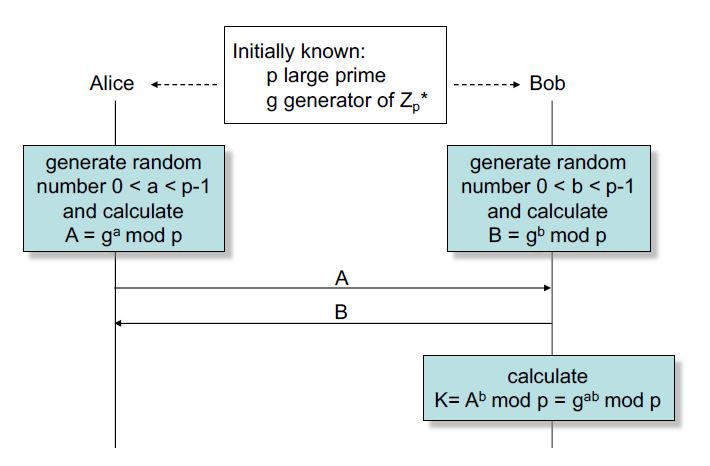
\includegraphics[width=0.50\textwidth]{C:/Users/Basti/git/Netzbasierte-Anwendungen-und-Dienste/diffiehellman.JPG}
	\label{fig:diffiehellman}
\end{figure}
\subsubsection{Zertifikate}
Zertifikat ist eine Datenstruktur welche folgendes enthält:
\begin{itemize}
	\item Öffentlichen Schlüssel
    \item Namen des Eigentümers des öff Schlüssels
    \item Namen des Ausstellers
    \item Ausstellungsdatum
    \item Ablaufdatum
    \item Möglicherweise andere Daten
    \item Signatur des Ausstellers
\end{itemize}
\subsubsection{Certification Authorities (CA)}
stellen Zertifikate aus.\\
sind normalerweise vertrauenswürdige Dritte.\\
Zertifikate werden über online Datenbanken verteilt(Certificate Directories) denen vertraut werden muss.
\section{Paketfilter}
 \subsection{Funktionsweise von Paketfiltern}
Netzwerkpakete werden akzeptiert oder zurückgewiesen anhand von Parametern wie:
\begin{itemize}
	\item Quelladresse/Ports
    \item Zieladresse/Ports
    \item Flags
\end{itemize}
\subsection{Paketfilterregeln}
Regeln können bzgl Flags, Adressen und Ports angewandt werden.\\
Paketfilter können auch bezüglich des Inhaltes von Paketen angewandt werden.\\
Zulassende Regeln:
\begin{itemize}
	\item explizites Erlauben von Zugriff
    \item sämtlicher anderer Verkehr wird verhindert
\end{itemize}
Verhindernde/ablehnende Regeln:
\begin{itemize}
	\item bestimmter Verkehr wird explizit abgelehnt.
    \item sämtlicher anderer Verkehr wird für gewöhnlich zugelassen.
\end{itemize}
Wichtig:
\begin{itemize}
	\item Reihenfolge der Regeln ist wichtig.(erst alles verhindern und dann einige zulassen ist was anderes als erst einige zulassen und dann alles zu verhindern!)
    \item große Anzahl an Regeln kann verwirrend sein.
    \item "`alles verbieten und solange es nicht explizit benötigt wird"' kann gute Herangehensweise sein.
\end{itemize}
\subsubsection{Ingress-Filter}
Filtern ankommende Pakete\\
blockieren Zugriff von verdächtigen Quelladdressen.\\
 \subsubsection{Egress-Filter}
Filtern ausgehenden Verkehr.\\
Nur Pakete mit Quelladdresse im Netzwerk dürfen das Netzwerk verlassen so lange keine andere Regel greift.\\
Quellen von abgewiesenen Paketen sind gute Kandidaten für Überprüfung.\\
\subsubsection{Protokollfilter}
Dienste haben haben festgelegte Protokolle\\
Daumenregel: nur Verkehr zu Diensten zulassen die wirklich benötigt werden.\\
\subsubsection{Probleme}
Zugriff für bestimmte Netze zulassen\\
Gefahr des Spoofings: Angreifer nutzt evtl falsche Quelladressen\\
Source Routing: 
\begin{itemize}
	\item Pakete enthalten evtl Infos über die Route zurück zum Urheber
    \item Überschreiben die Routingtabelle des Routers
\end{itemize}
Gefahr das Filterregeln umgangen werden\\
Fragmentierung:
\begin{itemize}
	\item Paketfilter untersuchen Headerinfos
    \item Paket wird so aufgeteilt dass der Header geteilt wird und Adresse und Ports nicht gefiltert werden können.
\end{itemize}
Löcher:
\begin{itemize}
	\item Dienste müssen erreichbar bleiben für externe Netzwerke
    \item entsprechende Ports müssen geöffnet werden.
\end{itemize}
\subsection{dynamische Paketfilter}
Filterregeln werden on the fly so erstellt wie sie benötigt werden und nach schließen der Verbindung wieder gelöscht.\\
Filter beobachten ausgehenden Verkehr und erstellen zurückwirkende Regeln.(Ausgehender Verkehr zu einer Adresse bewirkt Regel dass eingehender Verkehr von dieser Adresse erlaubt wird.)\\
Probleme: 
\begin{itemize}
	\item Regeln sind angreifbar z.B. durch senden falscher reset Pakete
    \item ausgehender Verkehr wird nicht gefiltert. Gefahr von Trojanern/Viren.
\end{itemize}
\section{Zustandsbehaftete Fierwalls}
\subsection{Funktionsweise}
Kennen den Zustand von Verbindungen und wissen welche Pakete in welchem Zustand erwartet werden.\\
Es können Regeln angewandt werden die nur in bestimmten Zuständen wirksam sind.\\
Untersuchen hauptsächlich  OSI 4 (transport layer), aber auch höhere Schichten.\\
\subsection{Probleme}
Hohe Leistung benötigt teilweise geclusterte Hardware. Zustandsbehaftete Firewalls lassen sich nicht einfach clustern.\\
Zustandslose Protokolle (UDP, ICMP, DNS, HTTP)\\
\subsubsection{Zustandslose Protokolle}
Zustandslose Protokolle definieren trotdem welche Pakete erwartet werden.\\
Timeouts werden genutzt um Pseudo-Verbindungen zu erzeugen.\\
\subsection{Multi-Layer Inspection}
Die meisten Protokolle basieren auf Protokollen aus niedrigeren Layern. BSP: HTTP nutzt TCP Verbindungen.\\
Zustandsbehaftete Firewalls können beide Layer beobachten.\\



\end{document}